\section{附录图表}

\subsection{描述性诊断补充图}

附录图 \ref{fig:app-event-rate} 补充报告压力事件率的时间变化，用于支持正文关于样本外事件不平衡的讨论。

\begin{figure}[H]
    \centering
    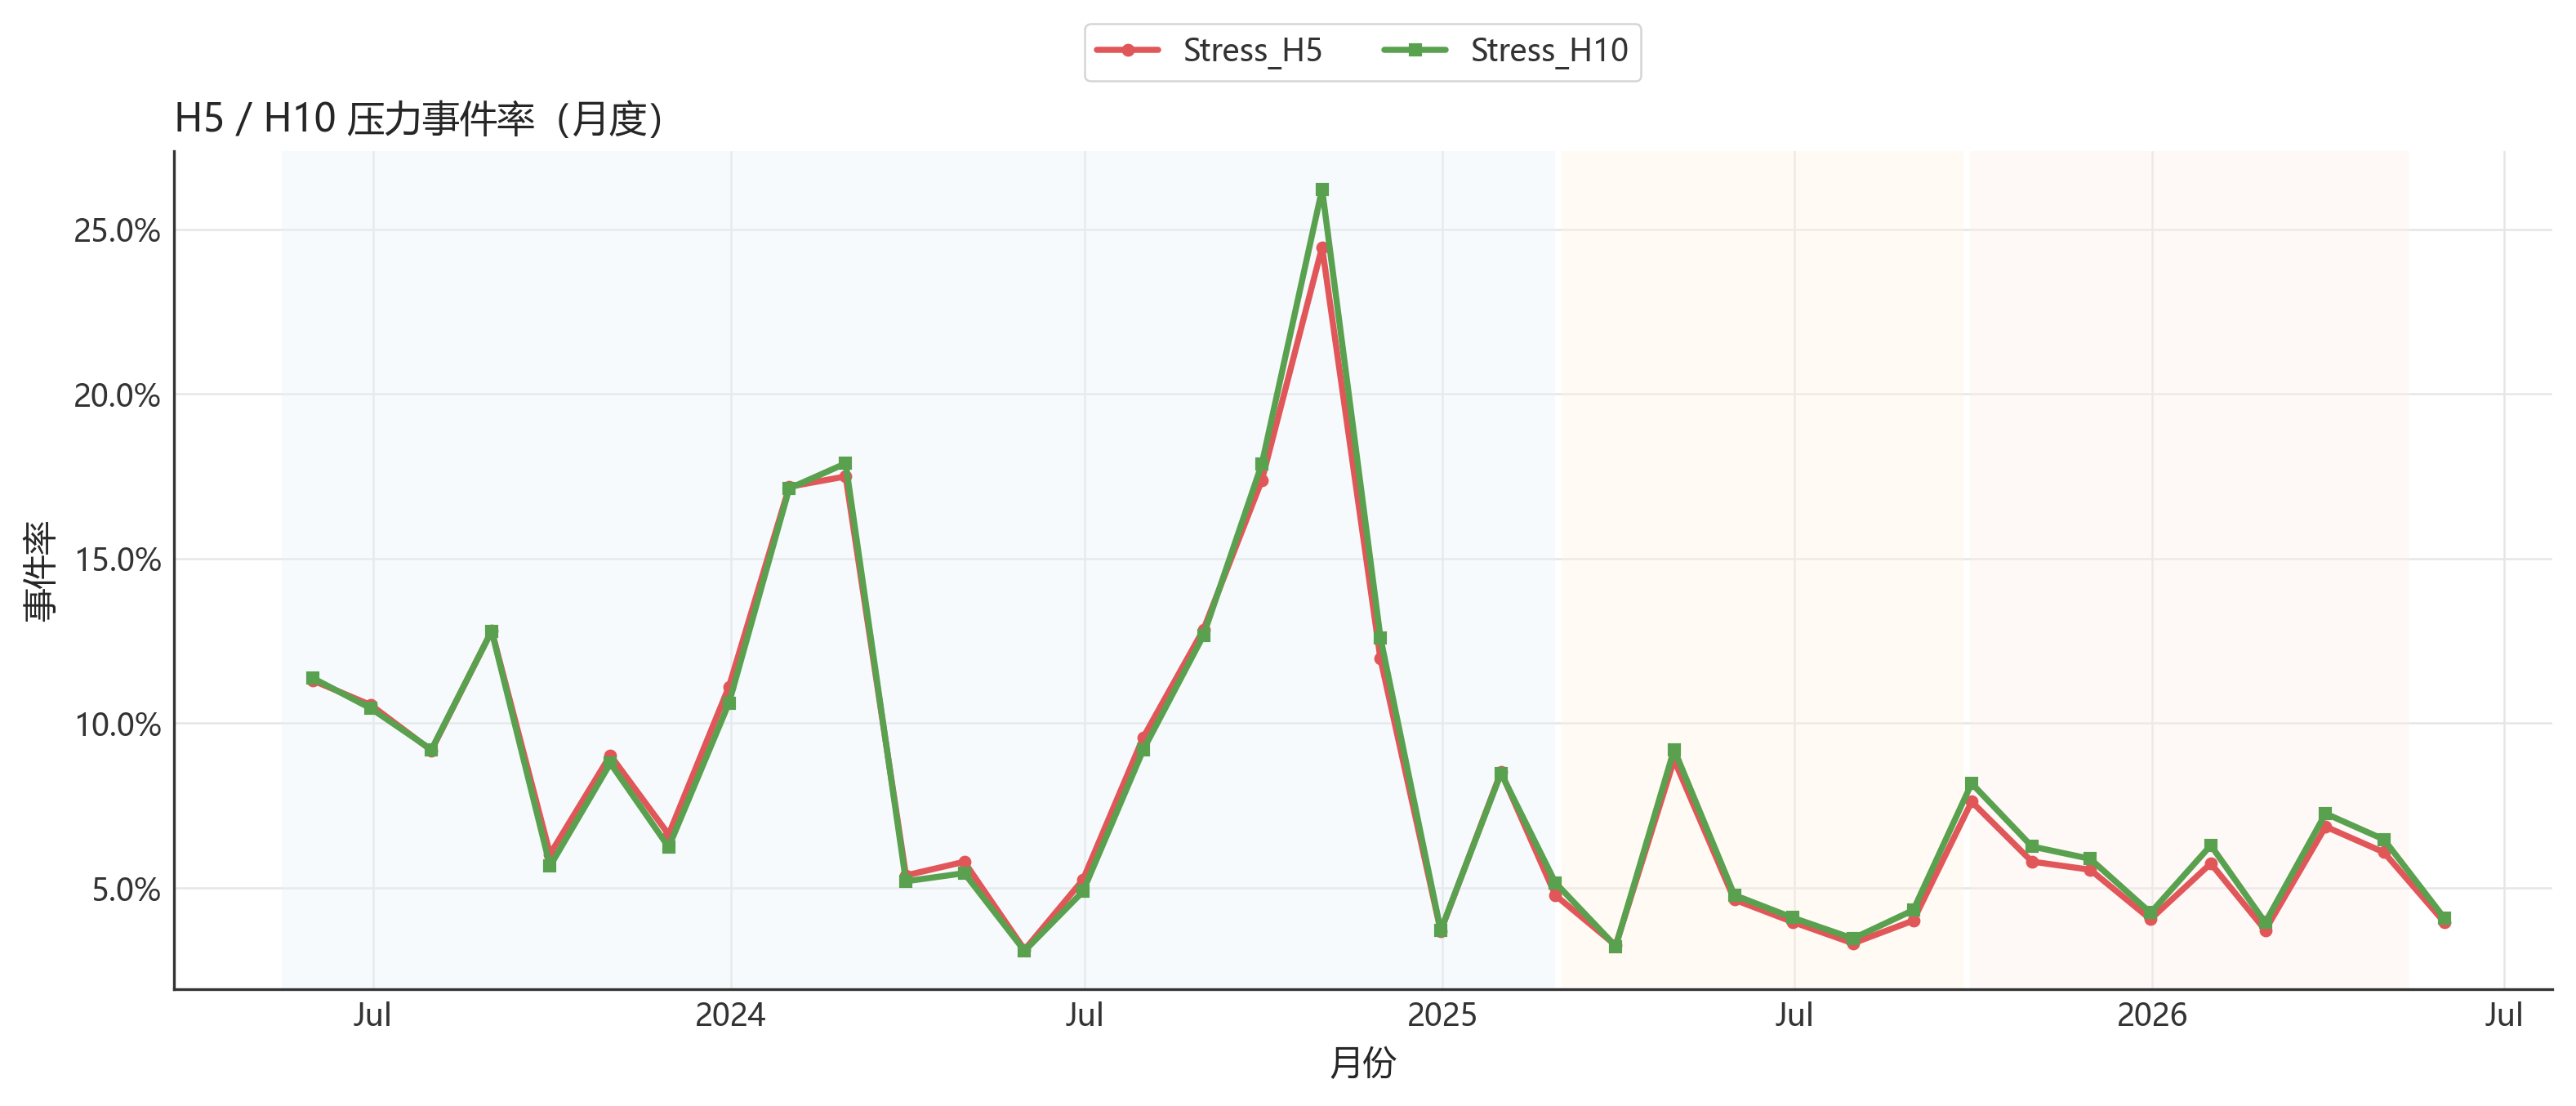
\includegraphics[width=0.88\textwidth]{figures/fig_event_rate.png}
    \caption{H5/H10 压力事件率时间变化。该图用于补充说明压力事件在训练、验证和测试阶段的时变性。}
    \label{fig:app-event-rate}
\end{figure}

附录图 \ref{fig:app-corr} 报告核心日度变量之间的线性相关结构，只用于背景诊断。

\begin{figure}[H]
    \centering
    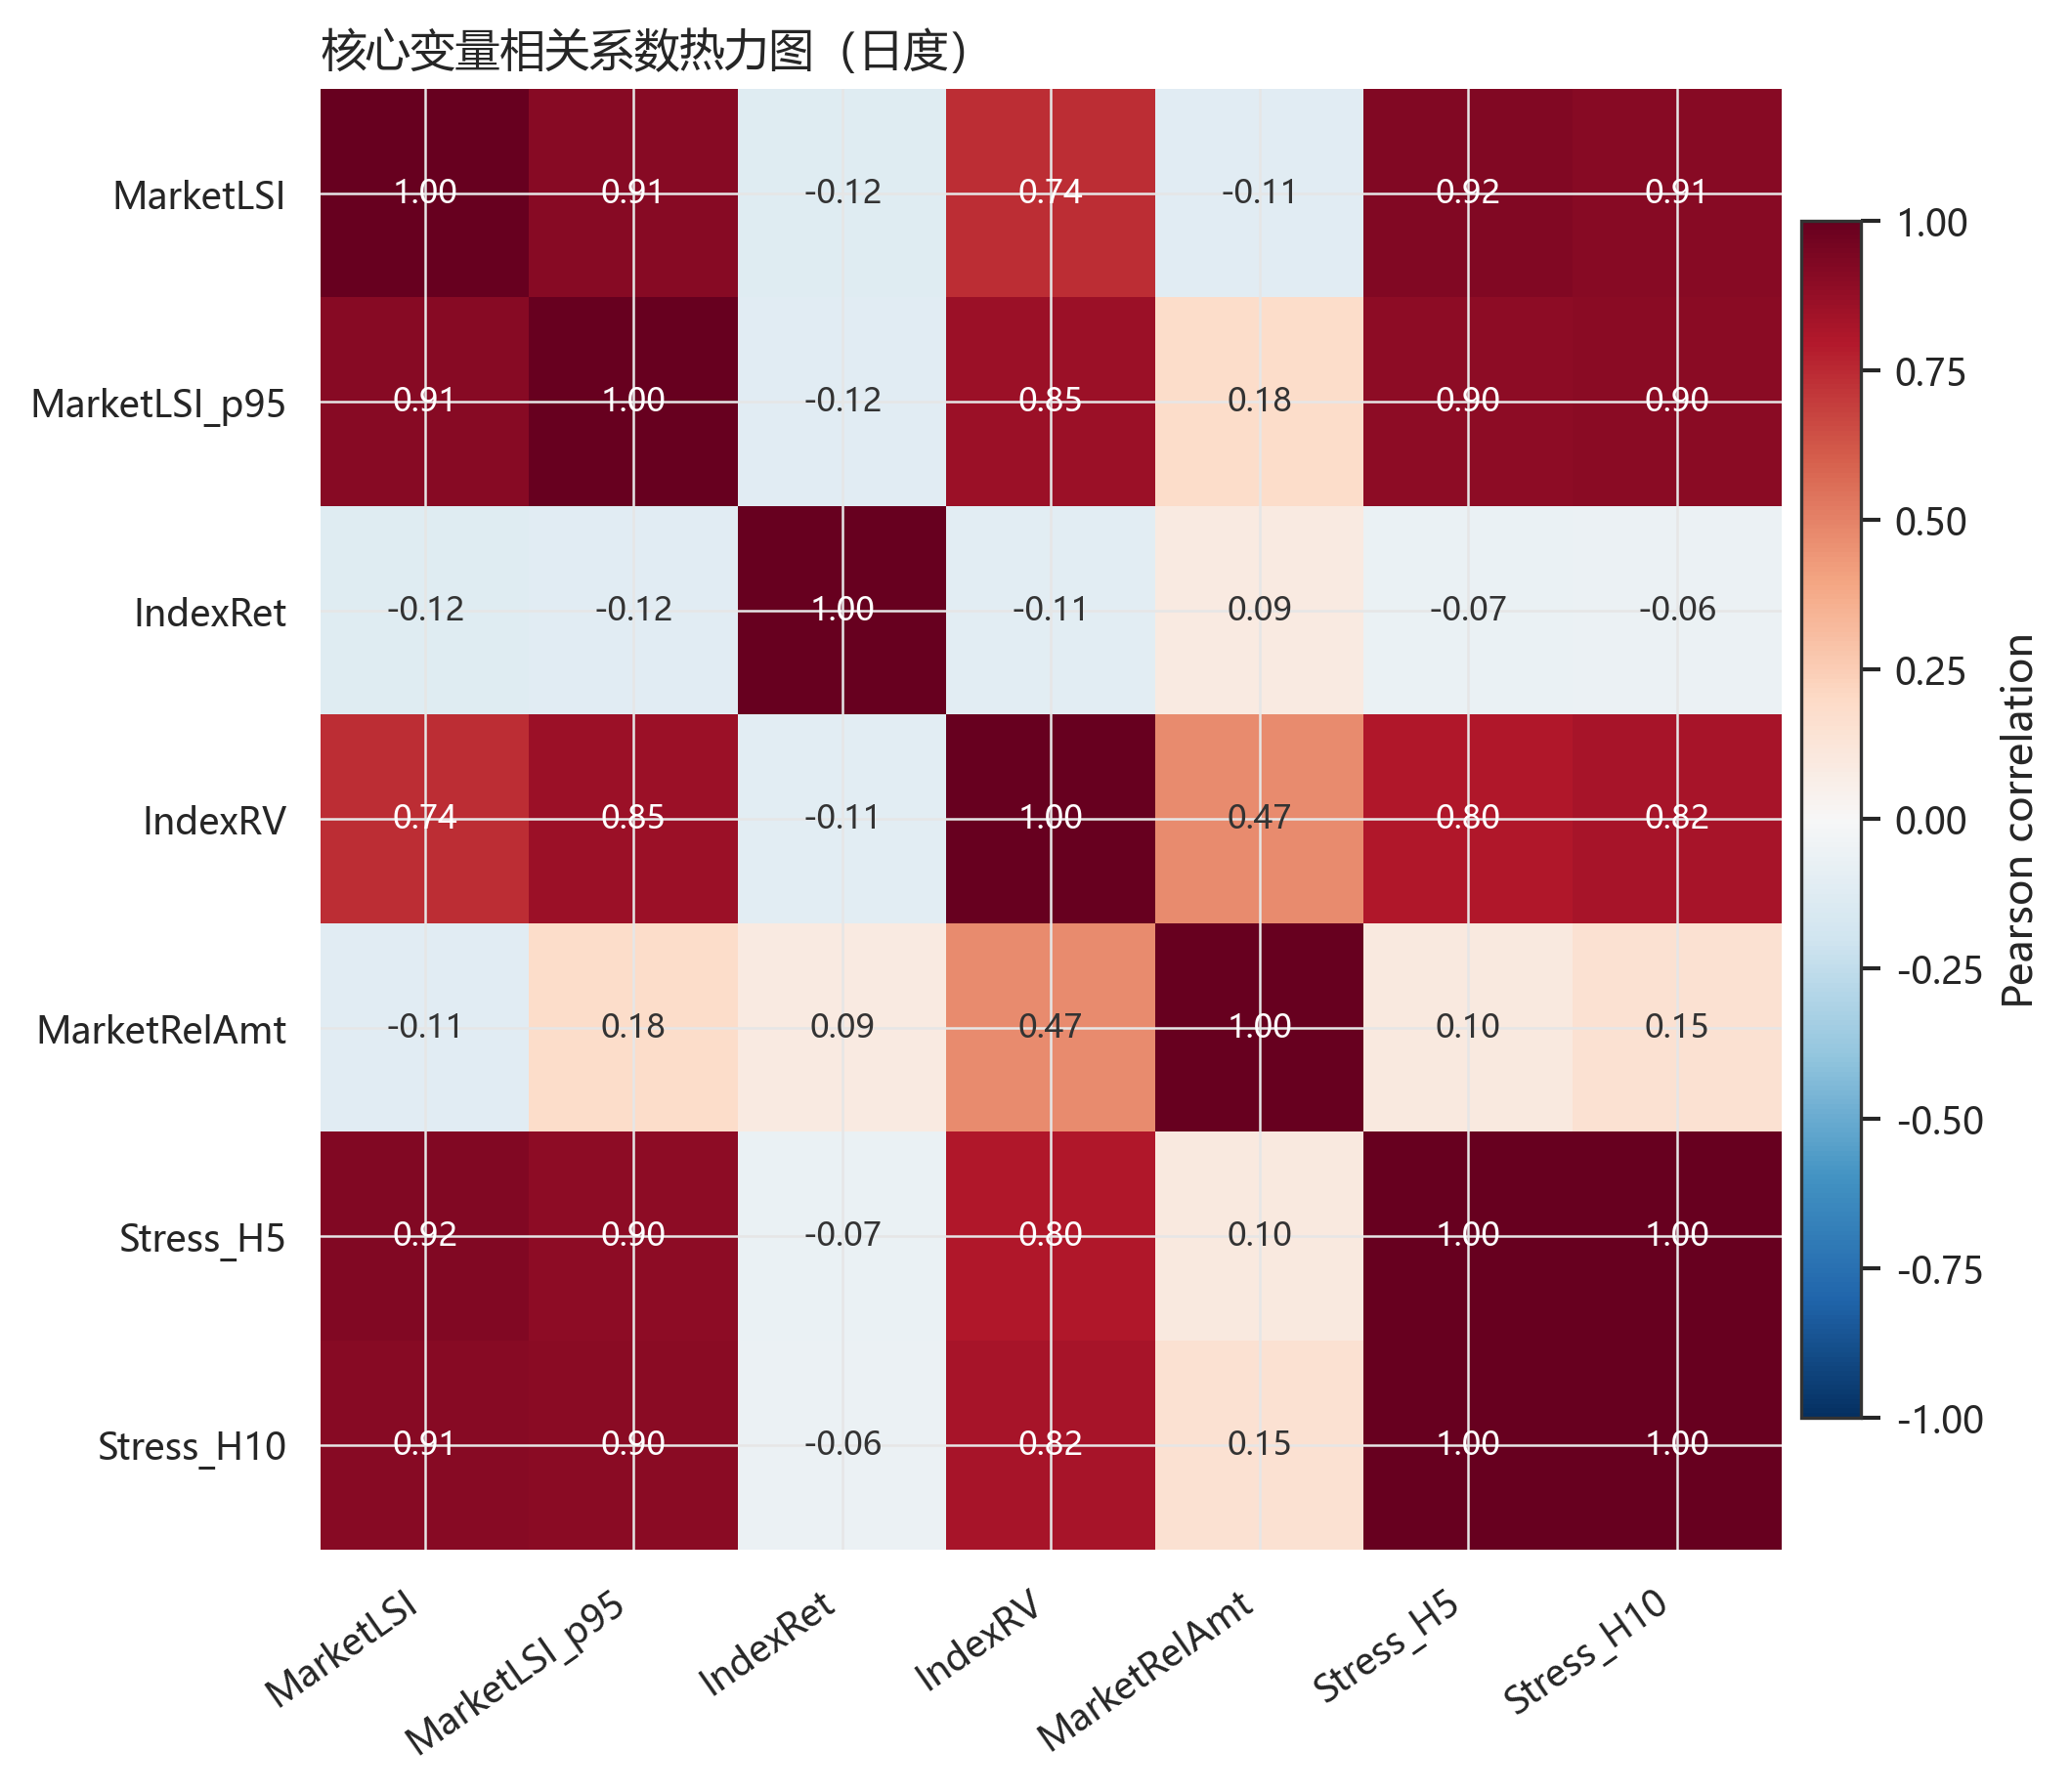
\includegraphics[width=0.76\textwidth]{figures/fig_corr.png}
    \caption{核心市场状态变量相关性热力图。相关结构仅用于描述变量共动，不构成因果识别。}
    \label{fig:app-corr}
\end{figure}

\FloatBarrier

\subsection{模型诊断补充图}

附录图 \ref{fig:app-sb-calibration} 补充查看 SMARTBoost 概率输出的校准表现。

\begin{figure}[H]
    \centering
    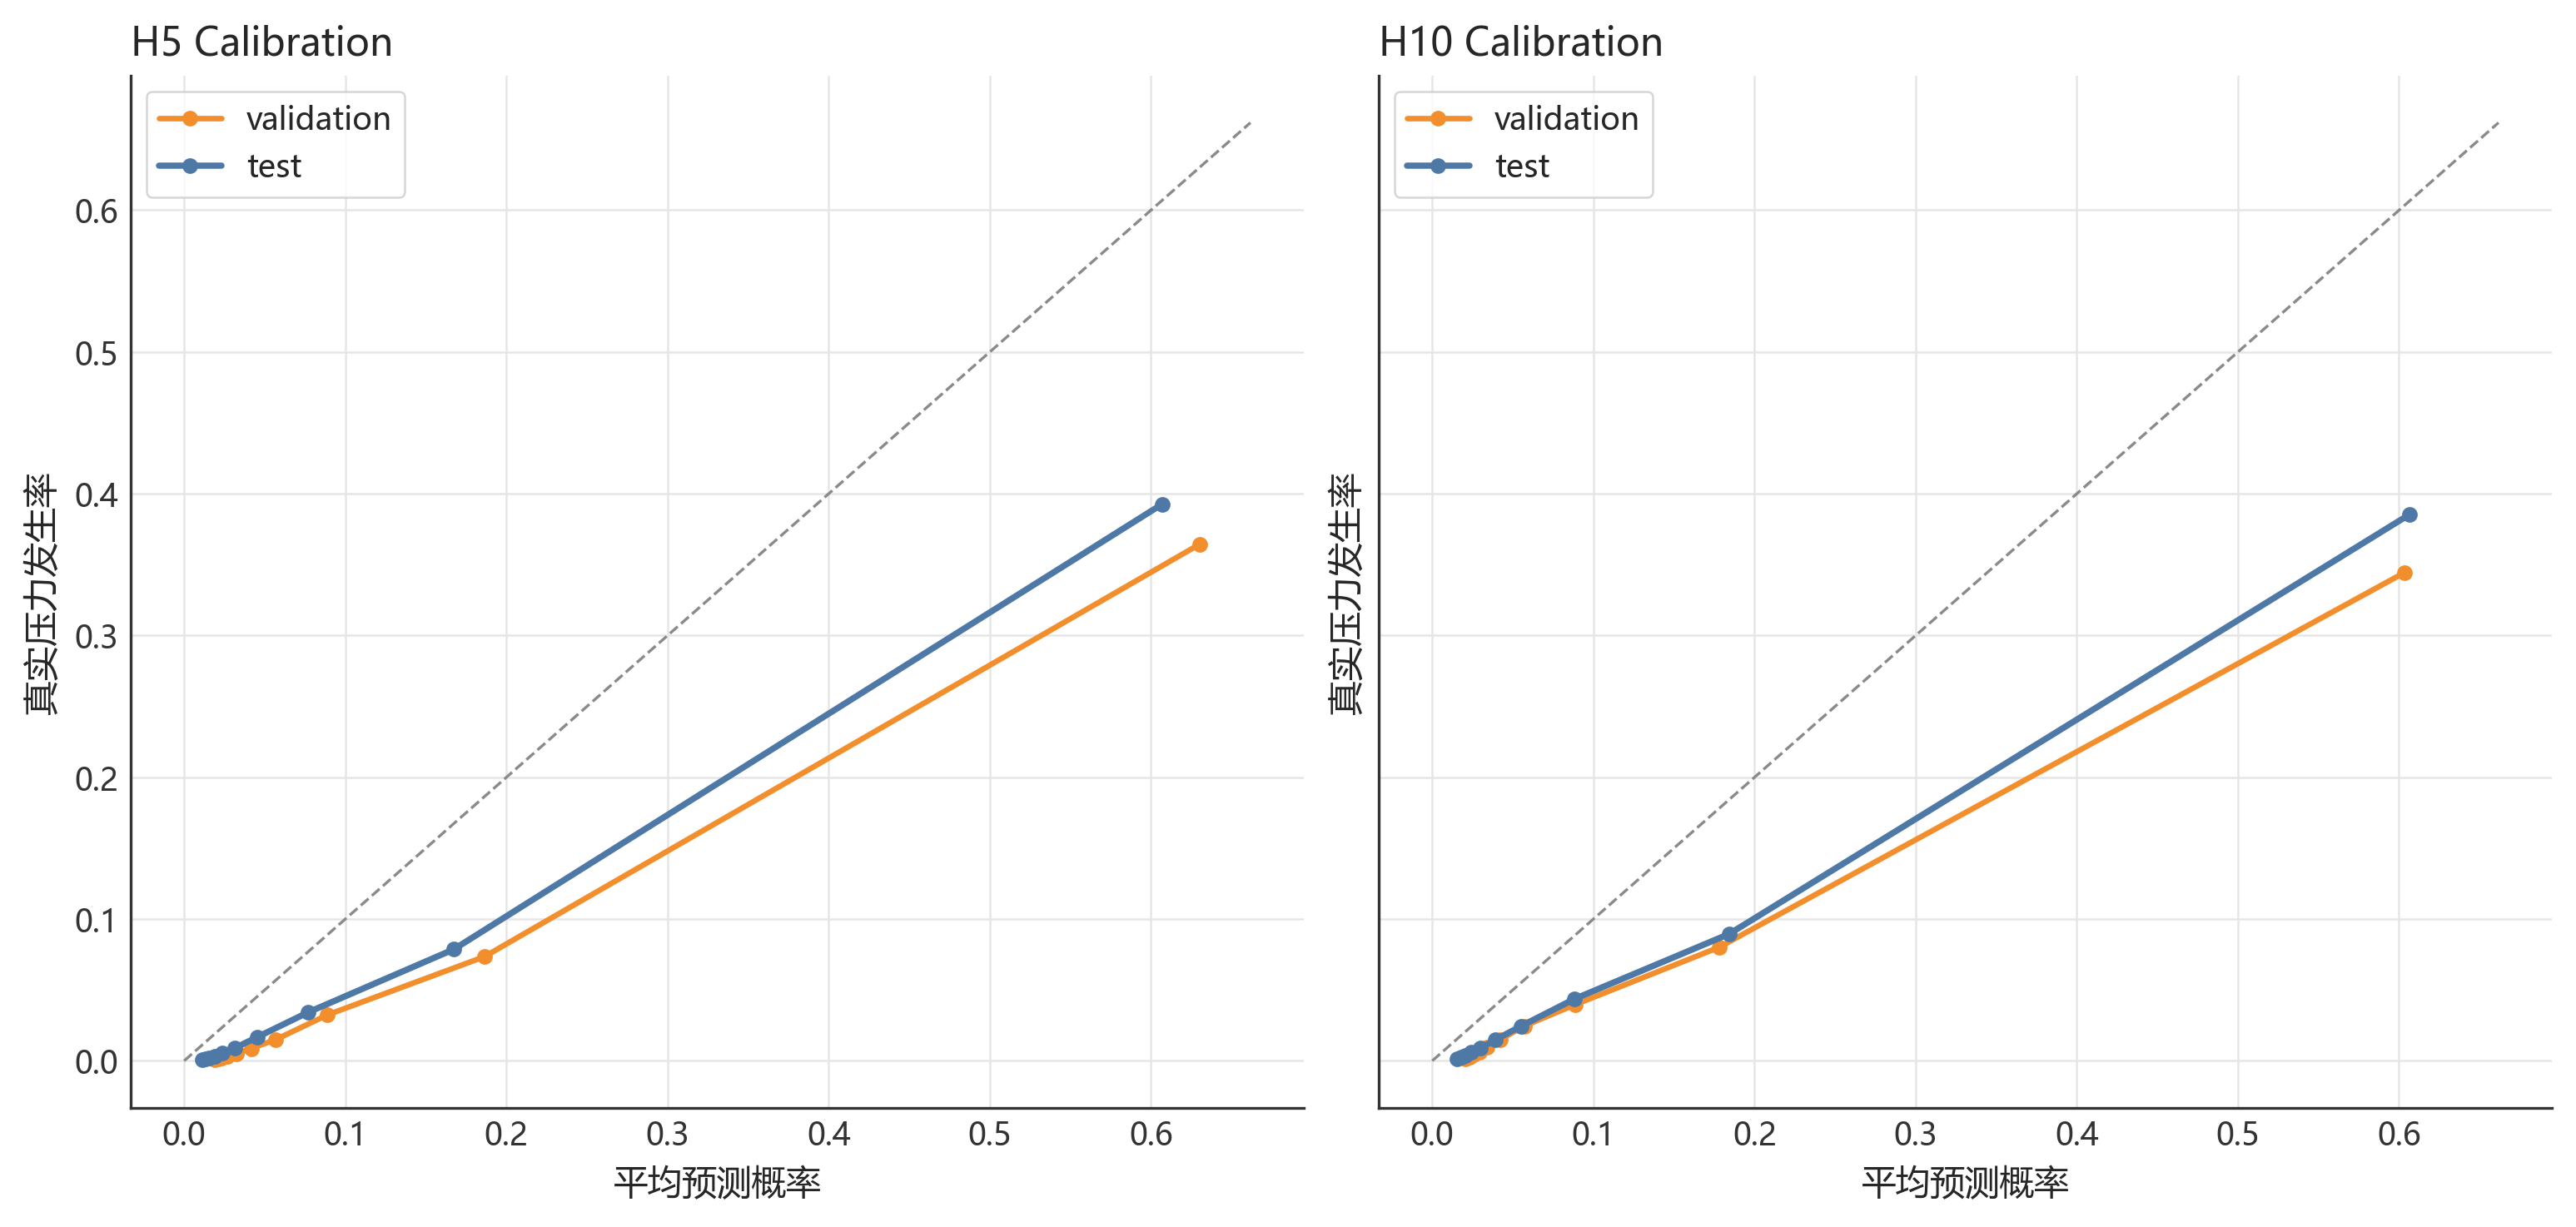
\includegraphics[width=0.86\textwidth]{figures/fig_sb_calibration.png}
    \caption{SMARTBoost 样本外校准曲线。该图作为 Brier 指标的视觉补充，不替代 PR-AUC 和高风险组命中率证据。}
    \label{fig:app-sb-calibration}
\end{figure}

\FloatBarrier

\FloatBarrier
